\begin{scanpage}{0072}{55}
\begin{center}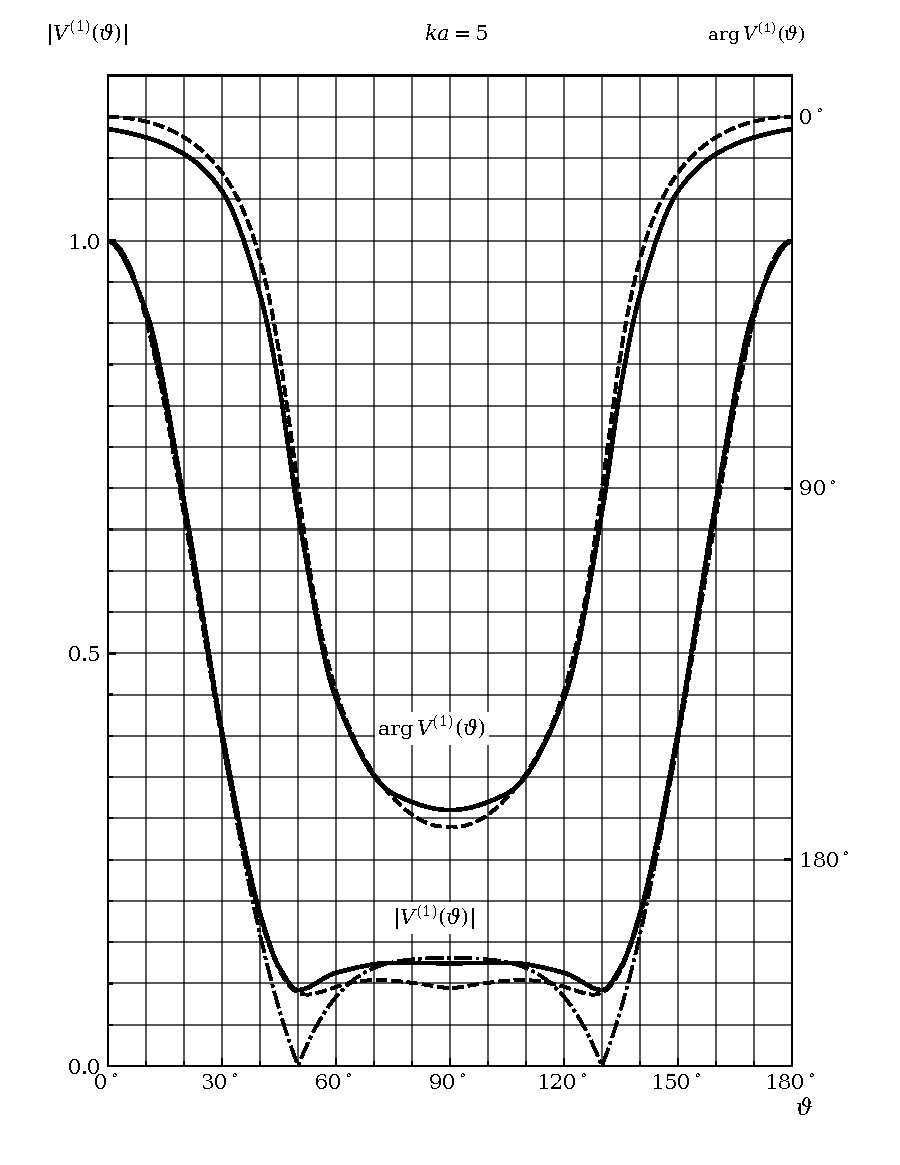
\includegraphics[height=11cm]{images/recreated/a-0072-fig20.pdf}\par Figure 20. The function $V^{(1)}(\theta)$ for a disk with a normal incidence of the wave. The various curves correspond to different approximations.\end{center}
The field radiated by it is found, as was done in \S\ 7, by integrating (with the condition $R\gg ka^2$). In the case of E-polarization of the incident wave $(\mathbf E_0\perp yoz)$, this field equals
\[\left.\begin{aligned}E_\theta=H_\phi&=iaE_{0x}\cos\gamma\cos\theta\cos\phi\frac{J_1(ka\sqrt{\lambda^2+\mu^2})}{\sqrt{\lambda^2+\mu^2}}\frac{e^{ikR}}R,\\E_\phi=-H_\theta&=-iaE_{0x}\cos\gamma\sin\phi\frac{J_1(ka\sqrt{\lambda^2+\mu^2})}{\sqrt{\lambda^2+\mu^2}}\frac{e^{ikR}}R.\end{aligned}\right\}\tag{10.03}\]
\end{scanpage}
